\documentclass{article}
\usepackage{graphicx}
\usepackage{color}
\usepackage[dvipsnames]{xcolor}

\usepackage{a4wide}
\title{RF readout in Silicon}

\begin{document}

\section{Intro} % (fold)
	\label{sec:intro}
	As Moore’s law begins to break down, new computational schemes will be necessary for improved computation performance.  Quantum computing is an exciting avenue that already boast algorithms that should provide speedups or perform tasks that are impossible on conventional computers.  Of the physical platforms available, spin based quantum bits (qubits) in semiconductors are particularly promising.  These qubits can be initialized quickly and with high fidelity through spin dependent tunneling to a neighboring fermi sea.  Single qubit gates with fidelities above 99\% and two qubit gates with above 90\% have been demonstrated.  The small size and localized nature of the control also lend themselves naturally to scaling to the number of qubits needed for a fully functioning quantum computer.   
	\\ \\
	Charge sensing is an important technique for measuring spin qubits because their long-lived spin states can be converted into more easily detectable charge states.  While this can be performed using DC measurements, it can be measured more quickly using high frequency techniques.  Radio Frequency (RF) reflectometry has proven to be a very effective technique in gallium arsenide (GaAs) spin qubits and has enabled single shot readout with only several microseconds of integration.  However, silicon germanium (SiGe) has proved to be a more challenging platform in which to implement RF reflectometry due to larger capacitances to ground.  Typical GaAs substrates are depletion mode while SiGe wafers are most often doped
	% \footnote{\color{blue}mostly SiGe is not doped, as it decreases strongly the mobility of the quantum well.}
	to be accumulation mode and require metallic electrostatic gates to cover all current paths so that the two dimensional electron gas (2DEG) can be populated.  This capacitive coupling between the 2DEG and gates is undesirable for RF reflectometry because it provides low impedance leakage pathways to ground that are independent of the sensor dot (SD) that is capacitively coupled to the qubit and used to detect the qubit charge state.  This reduces the sensitivity of the reflected signal to the qubit state.
	% \footnote{\color{blue}simpler (?) : due to the large capacitance of the gates with the 2DEG, it is hard to make a good matching circuit, as large capacitances lead to matching conditions with low resistances ($<100k\Omega$) and low frequencies ($<40MHz$).}
	The capacitance to ground is also dependent on the gate voltage because the capacitance is zero when depleted and finite when accumulated which provides additional difficulty when designing the measurement circuitry
	% \footnote{\color{blue} remove last sentence?}
	.
	\\ \\
	Here we demonstrate that RF reflectometry can be achieved in SiGe by reducing the capacitance of the device or by mitigating its effects.  There are two general approaches to reflectometry that differ in how the measured RF signal is carried to the lead of the sensor dot.  In the ohmic style, the signal enters the 2DEG through an ohmic contact so that it carried in the 2DEG itself all the way to the dot.  In the capacitive style, it is carried by a gate which is capacitively coupled to the lead in the 2DEG near the sensor dot.  We note that in both cases the sensitivity of the measurement is to the resistance through the quantum dot and not the quantum capacitance because the signal always enters the SD from the lead and not directly from a gate.  For both schemes careful care has been taken to reduce the effects of the capacitance on the sensitivity of tank circuit to the resistance of the SD and we discuss the different considerations that must be taken with each approach. 

\section{RF Reflectometry circuit and theory} % (fold)
\label{sec:rf_reflectometry_circuit_and_theory}

\subsection{Why SiGe is very different from the simples reflectometry} % (fold)
	\label{sub:why_sige_is_very_different_from_the_simples_reflectometry}
	In RF reflectometry, a fixed frequency signal is reflected off an impedance matching inductive capacitive (LC) tank circuit that is loaded with the SD, as shown in *(a).  The resistance of the sensor dot (RS) depends on the potential of SD which is very sensitive to it’s environment, and thus to the charge states in the nearby dots.   The reflection coefficient of this tank circuit is given by Gamma=(Z-50Ohms)/(Z+50Ohms), where Z is the impedance of the loaded tank circuit and the 50 Ohms is the impedance of the RF cables of the system.  At the resonant frequency Z=L/RsC0, where L is a lumped element inductor and C0 represents the total capacitance of the circuit board, a lumped element capacitor and the parasitic capacitance of the bond wires to the device.  Because the reflection is strongly modulated when Z is close to 50 Ohms, the tank circuit is designed with L and C0 chosen to yield Z=50 Ohms for the most sensitive Rs, typically 20 to 100 $k\Omega$
	% \footnote{\color{blue} is this correct for SiGe, we usually are somewhere in between 400k and 1M? (both Wisconsin en Delft devices)}
	.  The effective impedance seen by the reflectometry is then further simplified to Z = i2pifL + 1/(1/(=R2 + i2pifC0).   This matching occurs when Gamma= 0 at a resonant frequency of f=1/(2pi sqrt(LC0)) and a matching resistance R=L/50Ohms*C.  For GaAs, this simple model is sufficient to capture the observed behavior. 
	\\ \\
	In SiGe, the simple tank circuit model fails due to two other significant terms.  We must also consider the contact resistance (R1) and parasite capacitance (Cgate) between the 2DEG of the lead to the environment, which is dominated by capacitance to the lead’s accumulation gate.  This modified model is shown in figure $label$.  If the contact resistance (R1) and the parasite capacitor Cgate are small, this model reduces to the one previously described.  These changes are significant because the presence of these terms can cause the tank circuit’s reflection to be insensitive to the conductance. Careful analysis into the role of the parasitic capacitance is necessary to understand and mitigate its effects.  
	\\ \\
	\color{blue}In accumulation mode devices, as in SiGe, \color{black} an additional capacitance of ~1 pF is added between the lead 2DEG and the accumulation gate.  Figure 1 (a) presents the ohmic sensing scheme for a typical overlap style device.  A quadruple quantum dot is formed with the lower set of gates and two sensors are formed with upper gates.  Large accumulation gates control the accumulation of the leads from the ohmics to the quadruple and SD’s.  For SiGe specifically, the 2DEG of the source lead has a capacitance to the accumulation gates, which is represented by Cgate. This capacitor couples to ground through the line resistance
	% \footnote{\color{blue}lumped element on pcb not introduced.}
	(Rblock) and parasitic capacitor (Cself), which both provide additional pathways to ground. This shunts the signal to ground and reduces sensitivity to the SD. \color{blue} Additionally, an increased lead resistance due to lower mobility? And thus we need to be more careful in simplifying the model. \color{black}

% subsection why_sige_is_very_different_from_the_simples_reflectometry (end)
\subsection{Ohmic approach circuit and model} % (fold)
	\label{sub:ohmic_approach_circuit_and_model}
	In figure *(c) we present the circuit model for the ohmic approach.   
	\\ \\
	We note that this extended model also works for GaAs, where impedance matching works for reflectometry. The main difference between SiGe and GaAs is how much the parasite capacitor Cself and Cgate will play a role. While it is hard to reduce parasite capacitances, we can reduce their impact by increasing C0 on board. Another important aspect of designing the tank circuit is to ensure that it can achieve 50 Ohms impedance matching in a resistance range close to that of the sensor quantum dot.  This will ensure that the reflection off the loaded tank circuit will be sensitive to the resistance of the sensor dot.  This can be achieved by tuning the inductor.  
	\\ \\
	From previous measurements of frequency
	% \footnote{\color{blue} measurment not shown/unclear how determined?}
	, we estimate a constant $Cgate = 0.45 pF$ and $C0= 0.8 pF$ which cannot be ignored. In order to minimize the leakage of RF signal through the gate to ground, we place resistors between the gate wire bonds and the RC filters that are used for the DC lines. This improvement is limited by the remaining parallel pathway to ground with$C_{self}$. Then the total leak to ground can be simplified into an effective capacitor C*gate = 1/(1/Cgate+1/Cself) which we have found to still be around 0.2 pF. This modifies the circuit model, as shown in *(b) so that there is a capacitive pathway straight to ground that is independent of the SD.   
	\\ \\
	We now explore the parameters range where we can achieve matching. In figure $3a-b$ we examine the matching frequency and sensor resistance respectively as functions of L and C with fixed C*gate = 0.2 pF, and a contact resistance R1 = 3 kOhm.  The most important aspect of this figure is that there are large parameter regimes in which best matching cannot be achieved, shown in white.  We see that the parameters used as the beginning lie deep within this region (marked as blue). It is unsurprising that the tank circuit is very insensitive to the sensor resistance in this regime. The parameters marked as the red dot in is far from the boundary between the matching and non-matching regions. We find that the dependence of the frequency and matching resistance behave as they would for the naïve tank circuit model with modified parameter C*0 = C0 + Cgate and R2 = R-R1. Near the boundary, we find the best matching impedance can change by a factor of 10~100 with only 1\% change in C0 or inductor, and thus is not ideal for reusing the same board for different samples. This simulation provides a regime in which the frequency and matching resistance can be tuned by selecting the proper values of C0 and L for an existing device design.   
	\\ \\
	We further verify the model with a tunable R1 as plotted in figure 2(c). Parameters description...Add more description on what this R1 does ... When R1 = 0 then the model still can reduce to a standard tank circuit with C*0 = C0 +Cgate while a finite lead resistor will break this simplification. It is thus necessary to minimize the resistance of the lead path to the sensor, otherwise the tank circuit will still be device sensitive. 
	\\ \\
	\paragraph{Switch from effect on board to on chip } % (fold)
	\label{par:switch_from_effect_on_board_to_on_chip_}
	We note that the resonant frequency is low in 50 MHz where the (C0, L) is far from matching boundary. However most cryogenic RF components only works above 100 MHz, and detection chain also favors a small change in the working frequency. This requires small parasite capacitor and thus careful sample design. To explore the minimum requirement to enable our previous tank circuit setting, in figure 3c we show the effect of varying Cgate with a fixed C0 = 0.8 pF and R1 = 3 kOhm.  This plot shows that Cgate<<C0 have little effect on the matching condition as desired but that Cgate$\sim$12\% C0 the matching impedance is extremely sensitive to a tiny change in Cgate and thus very sample dependent. Once Cgate> 15\% C0 there is no best matching condition.  This requires us to suppress C*gate by half with the same lead resistance.
% paragraph switch_from_effect_on_board_to_on_chip_ (end)
% subsection ohmic_approach_circuit_and_model (end)
% section rf_reflectometry_circuit_and_theory_ (end)
\color{gray} (original delft intro)
	If one would want to speed up spin qubit experiments, the place the optimize would be the readout process. To readout a spin qubit, a conversion from spin to charge needs to be done. This is usually done by Elzerman readout and Pauli-Spin blockade readout. To detect a charge state, one can make use of a sensing dot or gate dispersive readout. In case of the sensing dot (SD), it can be used to detect electrons in close proximity ($d < \sim  300nm)$, as the current through the sensing dot will depend on the electrics field  of the electrons. For dispersive readout, a change in quantum capacitance is detected when an electron can jump from one quantum dot to another one.\\
	In this work we will be focusing on charge sensing with a sensing dot. A difference in charge occupation is detected by a resistance change of the SD. In other words, this translates into a problems of accurately measuring a resistance (range $100k\Omega$ to $5M\Omega$). To tackle this problem there are a few ways of doing it.\\
	The easiest way (and most commonly used) way is to use measure the current through the sensing dot with a amplifier at room temperature (e.g. with a JFET). In the same line of thinking, to reduce the noise temperature, people have also build amplifiers which work at base temperatures. The hard thing here is to convert the high impedance signal to a $50\Omega$ signal. This gives better results than room temperature amplification, but nowhere close the the theoretical noise limit.\\
	An alternate approach, which has been heavily used in GaAs quantum dot systems, is the use of what is called 'rf readout'. In this approach a RF signal is send to the sensing dot. Instead of current one now measures the reflection of signal at the sensing dot site. The reflection depends on the resistance of the sensing dot. Or formulated differently, a signal with an impedance $Z_0$ ($50\Omega$) is send down into the fridge. A matching circuit is build to convert $Z_0$ into $Z_1$ (e.g. $500k\Omega$). In other words, when the SD has a resistance of $500k\Omega$, all the signal is absorbed, where otherwise it will be (partially) reflected.\\
	In the  following sections, we will show several methods that allow one to form a good matching network that can be used for accumulation mode devices (in GaAs one has depletion mode devices. \\
	The main issue when trying to design a matching circuit for a accumulation mode device is the extra parasitic capacitance that is added by accumulation gate (large gate on top of the 2DEG, see figure 1a). The reason for this is, that if one has a large capacitance, one needs to compensate with a large inductance if one wants to keep the matching point at the same resistance ($Z_L = \frac{L}{RC}$). In conclusion, it is possible to match with a large inductor. This will cause the system to have a low resonance frequency ($\omega = \frac{1}{\sqrt{LC}}$). It is hard to find commercial amplifiers that work well below $10MHz$. For example, $R_{MATCH} = 200k\Omega$ and $C = 1pF$ results in $x KHz$.
	\\ \\
	To circumvent this problem, we propose the following approaches:
	\begin{itemize}
		\item Adding additional components on the PCB to compensate for large parasitics (fig 1\textbf{b}).
		\item Reduction of capacitance of the accumulation by moving the ohmics close and breaking the 2DEG (fig 1\textbf{c}).
		\item Use the large capacitance of the accumulation gate to your advantage, use a lead gate for the ohmic (fig 1\textbf{d}).
	\end{itemize}
	In method (a) -- @Harvard people description
	\\
	In method (b), 
	\\
	\color{black}
\begin{figure}
	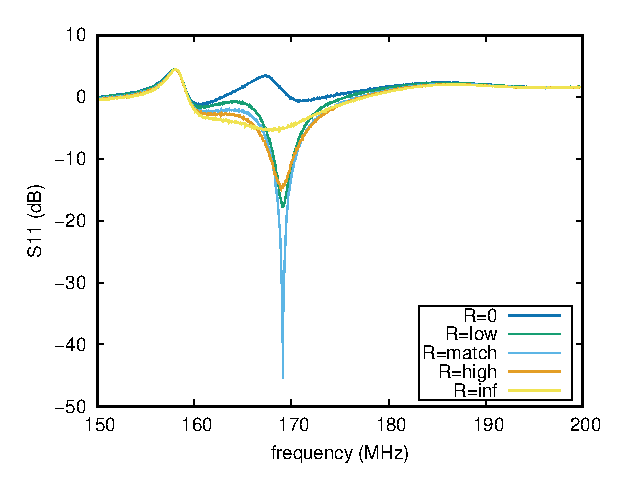
\includegraphics[width = \textwidth]{Illustrations/Overview/overview.eps}
	\caption{Circuit models for several device layouts with one sensing dot hooked up with RF readout on a mutilayer device type.  In the top image of each panel, a circuit model of the device is shown, in the bottom, a sketch of the physical device layout is shown. $L$ is the inductance of the inductor connected to the chip, $C_p$ is the parasitic capacitance of the inductor, the bondwire and the accumulation gate. In panel \textbf{(a)} a classical device layout is shown. In such a design the accumulation gate will have a large capacitance to the 2DEG below ($C_{2DEG}$). Panel \textbf{(b)} shows the circuit model and a schematic for the ohmic approach. In addition to the schematic in panel (a), a blocking resistor is added on the pcb to artificially reduce the effective capacitance of the accumulation gate. This resistor has as resistance $R_{block}$ and a capacitance $C_{block}$ (this capacitance is significant due to its macroscopic size). In panel \textbf{(c)}, the lead gate approach is shown, where the inductor is connected to the accumulation gate. This RF signal will couple in the 2DEG by the capacitive coupling of the accumulation gate. To make sure that the signal does not escape via the ohmic, a lead gate (see sketch) is added that allows to tune the resistance to the ohmic ($R_{Lead}$). In panel (d), an image is shown how the assembly of the inductor, resistor and lead gate looks like for the ohmic approach and a device image. Panel (e) shows a similar image for the lead gate approach.}
	\label{fig:overview}
\end{figure}
\subsection{Lead gate approach} % (fold)
	\label{sub:lead_gate_approach}
	\begin{figure}
		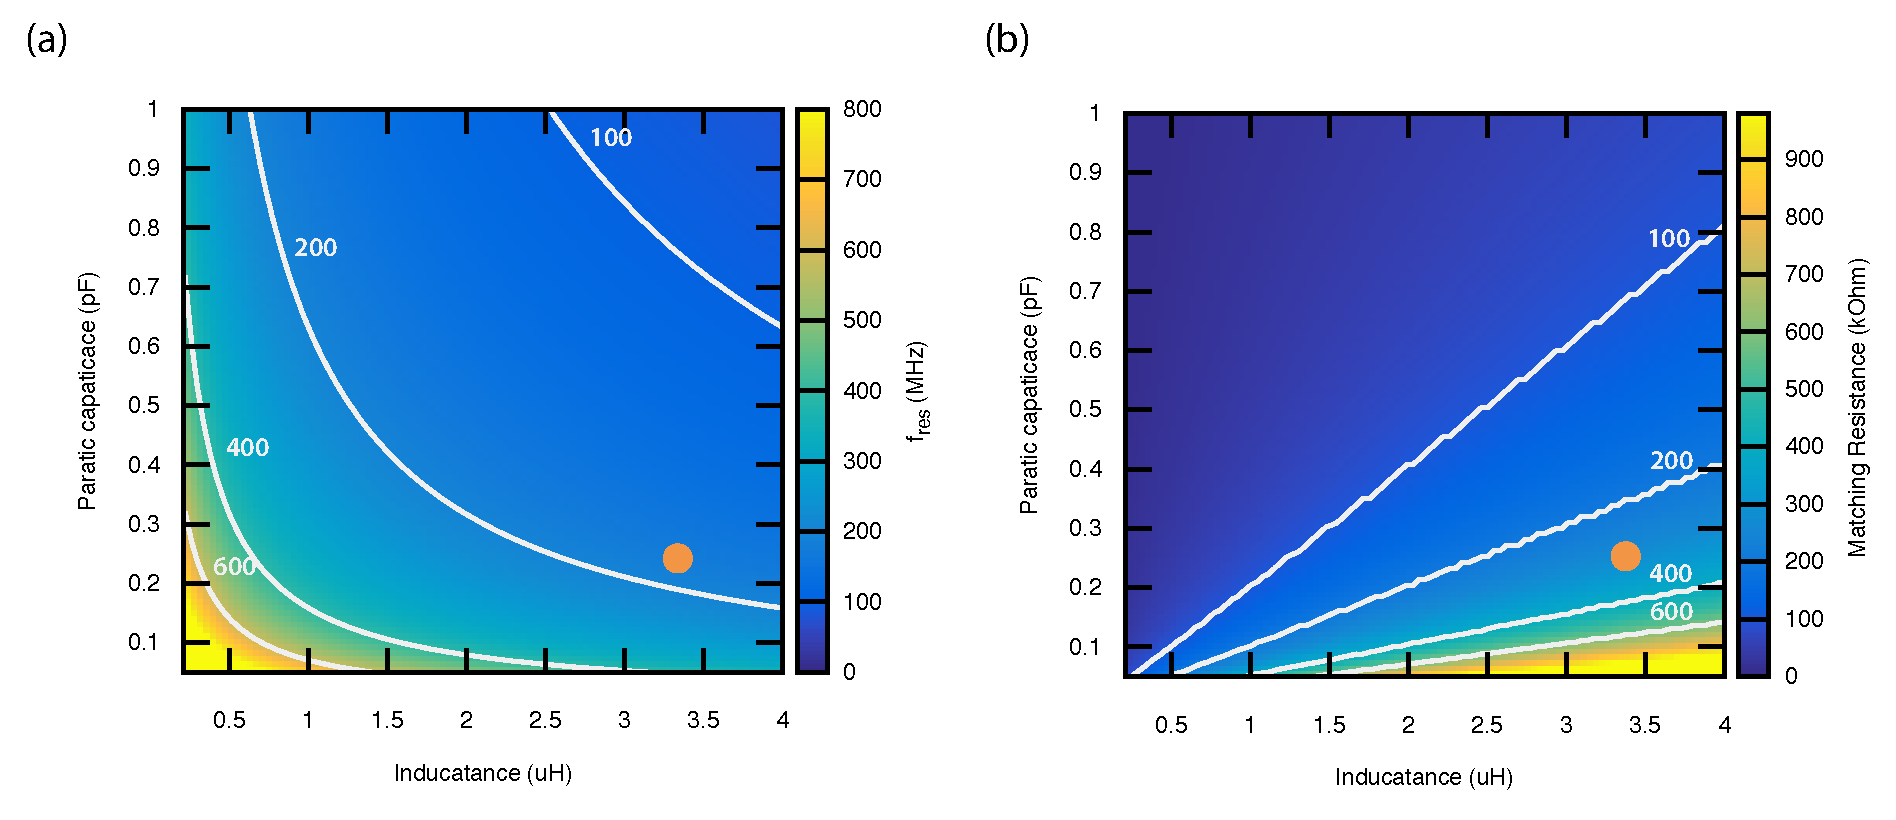
\includegraphics[width=\textwidth]{Illustrations/Theory_figure/theory_delft_v3.pdf}
		\caption{Circuit simulations for the circuit shown figure\ref{fig:overview}(c), where the inductance $L$ and the parasitic capacitance $C_p$ are varied. The resistance of the lead gate ($R_{lead}$) is set to $10M\Omega$ (typical value used in the experiment), the capacitance of the accumulation gate to the 2DEG is set to 1pF. The orange dot indicate the parameters for the device measured in this paper.}
		\label{fig:lead_gate_theory}
	\end{figure}
	In this approach, the RF signal (RF in) is applied via the second accumulation gate as shown in figure \ref{fig:overview}(c). The signal couples capacitively into the 2DEG ($C_{2DEG}$) and then travels to the sensing dot ($R_{sd}$). A large capacitance of the accumulation gate is desirable as it causes a low impedance for the signal to travel into the 2DEG \footnote{e.g. $C_{2DEG}$ of 1pF @ 200MHz has a impedance $< 1k\Omega$)}. From simulations we estimated that a capacitance greater than 50fF (@200Mhz) is needed to not effect the matching condition of the circuit.
	\\
	To ensure that the RF signal couples in via the accumulation gate and does not escape via the ohmic, the lead gate (fig \ref{fig:overview}(c)) is introduced.
	Its function is to make a variable resistor ($R_{lead}$) between the ohmic and the accumulation gate.
	When operated, its value is tuned $>>1M\Omega$ . We noticed that little difference is observed between operating the lead gate at $1M\Omega$ or open. This means it should possible to remove the ohmic all together, but this might make the tune up of the device harder, as no transport measurements are possible. \color{blue}relevant?\color{black}
	\\ \\
	To estimate what inductance is needed to generate a good matching condition, we performed a simple simulation of the resonant circuit. As boundary conditions we require that:
	\begin{itemize}
		\item The resonance frequency ($f_{res}$) that is greater than 40MHz (limited by the range of commercial amplifiers).
		\item A measurement bandwidth of $\sim 1MHz$ ($\sim$ 500ns rise time)
		\item Matching resistance ($R_{MATCH}$) between $100k\Omega$ and $1M\Omega$ (typical resistance range for a sensing dot in SiGe).
	\end{itemize}
	 In figure \ref{fig:lead_gate_theory}(a),  \ref{fig:lead_gate_theory}(b) and \ref{fig:lead_gate_theory}(c) we plot the resonance frequency, matching resistance and bandwidth for a given amount of parasitic capacitance ($C_p$) and inductance ($L$).
	 From the simulations, we see that there is a large parameter space where we fulfill the requirements set before. The most sensitive parameter is the matching resistance. The simulation indicates that one should to design a chip that has a parasitic capacitance lower than 400pF, if this requirement if fulfilled, one should be able to find an suitable inductor value that gives good RF readout performance.\\
	 In our case, the parasitic capacitance was around 250fF, where approximately 100fF originates from the bondwire and the remaining 150fF from the capacitance of the accumulation gate to the groundplane of the pcb. We used a superconducting high kinetic inductance inductor of 3.4uH to minimize self-capacitance of the inductor itself. The final matching resistance in our case is $275k\Omega$.  
% subsection lead_gate_approach (end)

\section{Results} % (fold)
\label{sec:results}
\subsection{Ohmic Style RF Reflectometry with modified on board elements} % (fold)
	\label{sub:ohmic_style_rf_reflectometry_with_modified_on_board_elements}

	Ohmic style RF reflectometry has been demonstrated in GaAs but the additional capacitances introduced by the accumulation gates have made reproducing this in SiGe challenging.  Here we demonstrate how to modify this scheme so that it is compatible with the accumulation mode devices that are used in SiGe.  We have identified four key strategies for device and circuit design that enable RF reflectometry in this system: blocking resistors, capacitance management on the PCB, LC tuning, and capacitance management on chip.  
	With this optimized board we first experimentally verify the tunability of the tank circuit performance on C0 and L. In figures 4a-c we show three different pairs of values with the same device and demonstrate that the matching resistance can be altered dramatically. We begin with the C0 and L as used in Figure 3(b), which used C*gate and R1 that is estimated from simulation shown in Figure 2 (a,b).  However we still find a frequency shift and matching at very resistive dot, indicating a larger C*gate or larger R1 than what is expected. The shift is gone with doubled C0 as demonstrated panel (b), but the matching condition is too conductive for a quantum dot. An ideal matching condition is shown in figure 4c with further increased inductor. In the end we achieve a best matching when the resonant frequency is around 34 MHz. Combining these three parameters we can extract a lead resistance R1 = 4 kOhm and C*gate = 0.45 pF. We note that this could be over fit since the parameters may vary between cool downs. 
	\\ \\
	In figure 3(c) another device of the same design is measured with the same tank circuit parameters and shows matching that is shifted up by 3\% and the matching impedance has increased by 40\%. This indicates a reduced C*gate by 3\% or a smaller R1.  Combined with the previous device, we did achieve the impedance matching with reasonable repeatability between devices.  We have noticed that even for a similar design the parameters are still device sensitive. We also note a 50\% change in the matching impedance when the inductor is changed by 10\% in the inductor, indicating we are still close to the edge of the matching regime in Figure 3(e). While we are able to drastically tune our matching conditions by using alternate tank circuit lumped elements, we find that the frequencies that we could achieve with this device design was lower than ideal as integration times will be longer for lower frequencies and RF components are less available. The final approach to improving tank circuit performance was improving the design of the quantum dot devices themselves.  
	\\ \\
	By narrowing the lead accumulation gates before the gate approaches the sensor, we were able to reduce the capacitance between the 2DEG and ground without reducing R1 too much.  This decrease of Cgate enabled the use of a significantly smaller C0 because, as shown in figure 3, it is the relative size of these capacitances that matters. From simulation we find C*gate is reduced by half, we used only the board capacitance of .8 pF and did not need to augment this with a lumped element capacitor.  To maintain the proper order of magnitude of matching resistance, the inductance was also decreased to 680 nH.  In figure 3 (d) we demonstrate that best matching can be achieved at 200 kOhm with a resonant frequency of 200 MHz, what can be achieved with commercial cryogenic RF components.  
	\\ \\
	However, this regime the tank circuit performance is very sensitive to the device. I.e, any change in R1, which is more dependent on the substrate 2DEG mobility, will change the best matching impedance or completely enters the no best matching regime. And even for devices fabricated with the same design, we need to change the on-board elements. To further study the impact on R1 and reduce the device dependent, we split the two gates. To achieve that we split the accumulation gate of the lead into two part: a ‘switch’ that turns on and off the connection from the Ohmic to the 2DEG and a channel that opens the electron path all the way to the sensor dot. The data is demonstrated in figure 3(d). With different gate voltage on the ‘switch’ gate, the total conductance through the dot is unchanged with the same voltages of all other gates, indicating a small back-action of this gate to the sensor tuning. In the contrast, the best matching is achieved with 1.5 nA for the fully accumulated switch gate, and 0.5 nA for a partial accumulated gate. The only difference between them is the larger R1 for partially accumulated switch gate and this agrees with the simulation in figure2 (c). With this tunable R1 we can somehow design the board elements with more general for different devices of the same design.
	\\ \\
	The tunable R1, however, is not the final solution because the larger R1, the more energy loss before the sensor dot, and thus smaller signal. To have a device insensitive tank circuit with enough signal to noise, we still need to reduce the self-capacitor as well as the contact resistance. One way to achieve that is to bring the Ohmic close to the dots, which reduce the metal area and shorten the distance of the lead 2DEG. Breaking the accumulation gates with a different design is another approach.

% subsection ohmic_style_rf_reflectometry_with_modified_on_board_elements (end)

\subsection{Capacitive Style RF Reflectometry} % (fold)
\label{sub:capacitive_style_rf_reflectometry}
In figure \ref{fig:lead_gate_result}(a), the response of the resonator is shown for several resistances (below and above the matching point). From this figure one can derive the bandwidth of the matching circuit. At matching point, the bandwidth is expected to be around 0.8MHz, this tells that the physical limit to detect a blib is around 600ns (assuming a perfect SNR). In general, when one increases the bandwidth, lower SNR is expected, as this will give a broadened resonance peak.
\\ \\
In panel (b) of figure \ref{fig:lead_gate_result} we characterized the reflectance of the matching circuit versus the resistance of the sensing dot. One can see that there are two highly sensitive regions, left and right from the matching point. In an ideal case, one jumps from the left to right side of the matching point (180 degree phase flip\footnote{FIGURE NEEEDS TO BE UPDATED TO PHASE AND AMP S11}). So in conclusion, for good design, we recommend to choose a matching point that is chosen to be right in the middle of your expected resistance range. In our case the the sensing dot was operated in a resistance range of 400$k\Omega$ to 1$M\Omega$. The current matching point is $275k\Omega$, we speculate that it would be possible to further increase the SNR of the circuit by decreasing the parasitic capacitance ($C_p$) of $250fF$ to $150fF$ (e.g. by making the footprint of the gates smaller (factor 3)) to match to $600k\Omega$.
\\ \\
Panel (c) and (d) of figure \ref{fig:lead_gate_result} show the performance one can expect from using this method. In (c) a charge stability diagram is shown. The acquisition time per point is set to 2us. This means that this readout is quite suitable for video mode tuning with high resolution ($>100\times100px$). In figure (d) we show the performance of the charge readout. There are two transitions probed. One is going from the top to the bottom of the coulomb peak of the sensing dot. From this measurement we should not be limited by the SNR and be able to measure the bandwidth of our system. We see that the charge readout fidelity strongly increases around 600-800ns blib size, as expected from the bandwidth measurement of the sensing dot. To probe practical readout performance, we measured the charge fidelity of a dot reservoir transition. In this case the readout is not bandwith, but SNR limited. For this particular transition (see fig \ref{fig:lead_gate_result}(c)), we expect 99.9\% charge fidelity of the readout in 2us.


\begin{figure}
	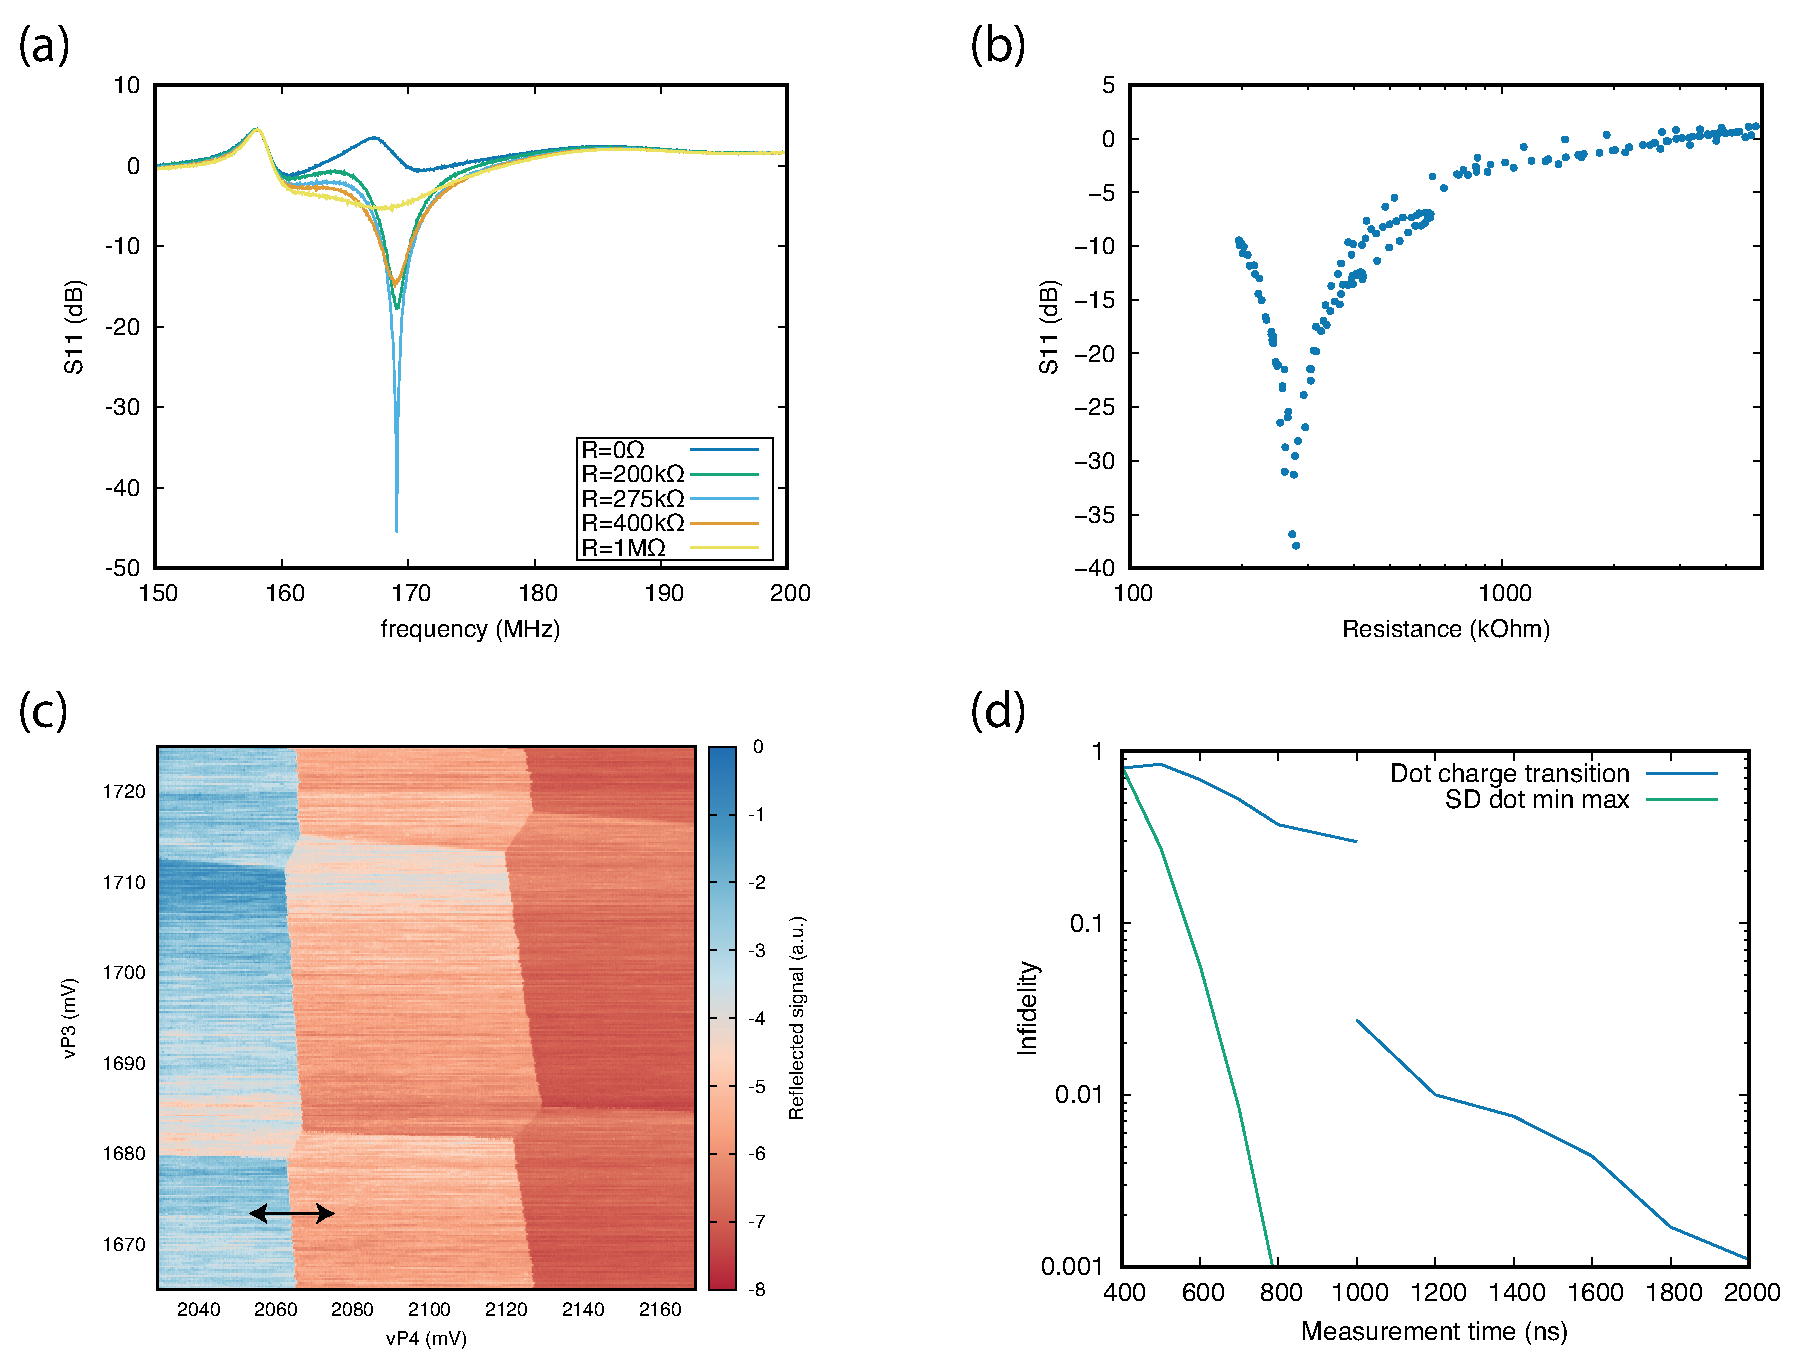
\includegraphics[width = \textwidth]{Illustrations/Performance_figure/performance.eps}
	\caption{Characteristics and performance of the lead gate approach. In panel (a), the response of the matching circuit to a change in resistance of the sensing dot is shown. The bandwidth of the circuit is expected to be ~0,8MHz from fitting the curve around the matching point.
	Panel (b) shows the response of the LCR circuit at the resonance frequency versus the resistance of the sensing dot. The circuit matches at 275kOhm.
	Panel (c) shows a charge stability diagram of dot 3 and 4, measured via rf readout (2us per point). The black line in the figure shows the transition that is probed in panel (d).
 	Panel (d) shows the infidelity of the charge detection versus time. The green line shows the fidelity of when going from the top to the bottom of a Coulomb peak of the sensing dot. The blue lines shows the fidelity for detecting a dot reservoir transition with a given length. The infidelity of the charge readout was estimated by sending a block pulse to the sensing dot or the quantum dot. When changing the frequency, one can check if it is possible to still differentiate the two signals generated by the block pulse (top and bottom). The fidelity is estimated by making a histogram of both signal and calculating the overlap (similar to how one would do it for qubit readout).
	}
	\label{fig:lead_gate_result}
\end{figure}
	
% subsection capacitive_style_rf_reflectometry (end)
% section results (end)
\end{document}